\begin{savequote}[8cm]
  ``I just wondered how things were put together.''
  \qauthor{Claude Shannon}
\end{savequote}
\makeatletter
\chapter{Experiments and Results}

\section{Experiments}

This section discusses the types of experiments performed. First, a survey on codec evaluation and comparison techniques is presented, then those techniques used to evaluate the SOT are reported. Next, the experiment environment used is discussed, along with the data set used in experiments.

\begin{figure*}[t] 
        \centering
        \begin{subfigure}[b]{2.0in}
                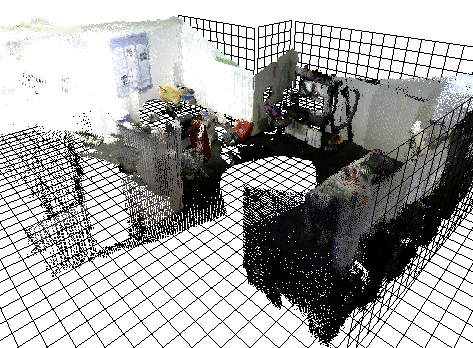
\includegraphics[width=2.0in]{images/ch2/unit21}
                \caption{Apartment}
                \label{fig:RECON_UNIT}
        \end{subfigure}%
        \begin{subfigure}[b]{2.0in}
                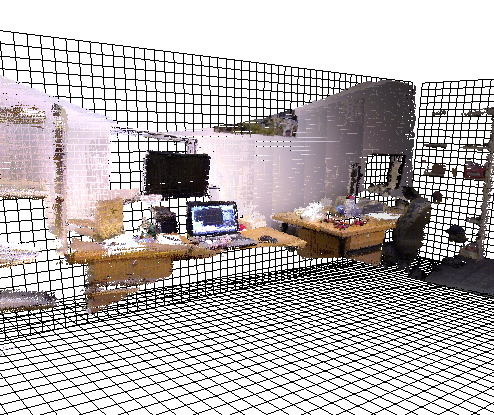
\includegraphics[width=2.0in]{images/ch2/officeA}
                \caption{Office}
                \label{fig:RECON_OFFICE}
        \end{subfigure}%
        \begin{subfigure}[b]{2.0in}
                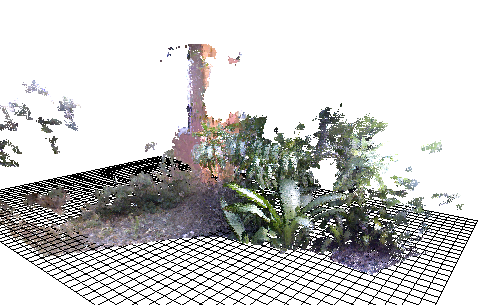
\includegraphics[width=2.0in]{images/ch2/outdoorA}
                \caption{Garden}
                \label{fig:RECON_GARDEN}
        \end{subfigure}
       \caption{Reconstructed Scenes.}
       \label{fig:RECONSTRUCTIONS}
\end{figure*}


\subsection{Codec Evaluation \& Comparison Techniques}

Codec evaluation involves comparing storage requirements between the original model and codec output. In the case of lossy codecs, a quantitative quality metric is also required. Compression metrics are easy to compute, quality metrics are more involved and there have been many proposed techniques. Quality metrics compare the distortion created by the codec relative to the original model. Two measurements are usually performed, the distance from the compressed model to the original and the distance from the original to the compressed model. Quality metrics are split into empirical and perceptual based metrics. Empirical metrics measure geometric error and perceptual metrics estimate human perception. Perception based metrics are a part of psychophysics research. For a more in-depth survey of these methods, see work by Bubill \textit{et al.} \cite{Bulbul11Assessing}.

\subsubsection{Compression Metrics}

In the context of 3D model compression, the file size of both, the compressed model and the original are compared. Alternatively, the file size of the compressed model from one codec can be compared to the file size of the same model compressed using another codec. The compression ratio ($CR$), defined as the original file size divided by the compressed file size, is a measure of compression performance. Another metric used is called the bit rate, different bit rates are used depending on the representation being compressed. The mesh representation uses bits per vertex (bpv) and bits per triangle (bpt), the volumetric representation uses bits per voxel and the point cloud representation uses bits per point.

\subsubsection{Empirical Error Metrics}

The following metrics are used to assess the error between two data samples. For two points, $p$ \& $q$, in $\Re^3$ space, the basic euclidean distance metric,
$$
ED(q,p) = \sqrt{(q_x - p_x)^2 + (q_y - p_y)^2 + (q_z - p_z)^2}
$$,
the absolute error,
$$
AE(q,p) = \|q_x - p_x\| + \|q_y - p_y\| + \|q_z - p_z\|
$$
and the squared error $SE$, 
$$
SE(q,p) = (q_x - p_x)^2 + (q_y - p_y)^2 + (q_z - p_z)^2
$$
are often used as a basis for other metrics. 3D models can be sampled into a set of points in $\Re^3$. Using these samples, the following metrics can be used: sum of distances ($SOD$), sum of absolute differences ($SAD$), sum of squared errors ($SSE$), mean square error ($MSE$) and root mean square error ($RMS$). Since the two models may be sampled differently, the minimum error from one sample to the others is used. These metrics are defined below using two point sets, $A$ \& $B$ where the length of these sets is $M$ and $N$ respectively.
$$
SOD(A,B) = \sum_{k=0}^{M} \min_{b \in B}(ED(A_k,b))
$$

$$
SAD(A,B) = \sum_{k=0}^{M} \min_{b \in B}(AE(A_k,b))
$$

$$
SSE(A,B) = \sum_{k=0}^{M} \min_{b \in B}(SE(A_k,b))
$$

$$
MSE(A,B) = \frac{1}{M}SSE(A,B)
$$

$$
RMS(A,B) = \sqrt{MSE(A,B)}
$$

For each of these metrics, $METRIC(A,B) \neq METRIC(B,A)$. Therefore, these methods are often averaged (below). This is termed the average metric (AM), as opposed to the minimum metric (MM) which is the smallest value of the two.

$$
AvgError = \frac{Metric(A,B)+Metric(B,A)}{2}
$$

Another metric, the Hausdorff distance ($HD$) is a measure of overall shape similarity. It is defined as the largest value of the maximum distances between objects from $A$ to $B$ and from $B$ to $A$. For example, for two objects $A$ \& $B$, the Hausforff distance $HD$, from $A$ to $B$, is defined as,
$$
HD(A,B) = \max(D(A,B),D(B,A))
$$
where $D(A,B)$ is defined as,
$$
D(A,B) = \{a \in A \| \max(dist(a,B)\}
$$
and $dist(a,B)$ is defined below.
$$
dist(a,B) = \{b \in B \left| \min(\|a-b\|)\right.\}
$$

\subsubsection{Human Perception Based Metrics}

Lavoue \textit{et al.} \cite{Lavoue06Perceptually} devised a metric based on structural distortion, this method correlates well with human perception. It is based on the SSIM method of Wang \textit{et al.} \cite{Wang04Image}, which is a popular image metric. Lavoue \textit{et al.} call their method the, Mesh Structural Distortion Measure (MSDM). An updated version of this metric was also developed \cite{Lavoue11Multiscale}.

\paragraph{Laplacian Metric}

Karni \& Gotsman \cite{Karni00Spectral} developed their own on-line metric for use during their spectral based codec. It is based on the laplacian and measures the difference between two objects in terms of their smoothness. 

\paragraph{Elastic Deformation Based Metric}

Bian \textit{et al.} \cite{Bian09Evaluation} developed a novel metric, useful for both on and off-line model comparison. The algorithm is based on the theory of strain fields. A strain field is a metric derived from elasticity, it is used to describe the deformation of some object which has elastic properties. Using this concept, both models are treated as having elastic properties in order to perform quality assessment.

\paragraph{Saliency Based Metrics}

Howlett \textit{et al.} \cite{Howlett04Experimental} and Lee \textit{et al.} \cite{Lee05Mesh} both presented work aimed at determining salient features in 3D models. They incorporated these findings in their own metrics. Howlett \textit{et al.} used a human gaze detection device to study the psychophysical effects of viewing 3D objects. Both of these metrics are based on preserving the sections of the object in which any distortion would be visibly noticeable to humans.

\paragraph{The Depth Difference Metric}

Krivokuca \textit{et al.} \cite{Krivokuca12New} developed a perceptual based metric for the off-line quality assessment of 3D models. This method is independent of model representation and is based on generating multiple depth maps from different orthographic perspectives. It improves upon both the Hausdorff distance and RMS error and is good at detecting both small and large geometric errors. Krivokuca \textit{et al.} call their method, the Depth Difference (DD). It works by comparing orthographic depth maps from both the original and compressed models. First a difference depth image is calculated ($DDI$) from orthographic depth maps of the original object ($DIO$) and of the compressed object ($DIC$). The $DDI$ is calculated using element-wise matrix subtraction,

$$
DDI = DIO - DIC
$$

Then the average depth distance value ($ADD$) is calculated from the $DDI$ matrix, this equation is presented below.

$$
ADD = \frac{1}{MN} \sum_{y=0}^{M} \sum_{x=0}^{N} DDI_{y,x}
$$

This $ADD$ value is then summed up and averaged over different orthographic views, this average is the Depth Difference.

\subsection{Codec Performance Assessment}

The experiments performed use a number of different metrics to quantify the performance of the SOT and compare it with other codecs. The quality metrics used include: mean distance, $RMS$, Depth Difference ($DD$), $MSE$, and qualitative perception. Most research uses the $MSE$ and $RMS$ because they are simple and provide an accurate measurement of quality. Since the data which the SOT is manipulating was designed for human visual consumption, the perceptual metric, DD is used. Our implementation of the DD metric uses five orthogonal projections corresponding to the sides of a cube (excluding the bottom face). Qualitative comparisons are also used to provide insight into the visual quality of the models which the SOT produces. The storage metrics used include: number of bytes and bpv. Bits per vertex is used most often because the input and output of the SOT is a polygonal mesh, and because it is widely used in the literature as part of rate-distortion graphs.

Results provided for the OT use the MM and results for the SOT use the AM. This is because the SOT can represent both outside and inside views of the mesh, whilst the OT can only represents the outside view. All measurements are computed using a $512 \times 512 \times 512$ bounding box, but when comparing the SOT with other codecs, the error is converted to the same bounding box used by the other codec.

\subsubsection{The Metro Program}

In order to ensure the accuracy of geometric errors, the Metro software tool is used to independently assess the quality of models produced by the SOT. This tool takes two models as input and produces the forward and backward $RMS$, mean distance and Hausdorff distance between the two. Metro Version 4.06 was used in all experiments, details about this software can be found in work by Cignoni \textit{et al.} \cite{Cignoni98Metro}.

\subsection{Experiment Environment}

All experiments were performed on an ASUS computer with an Intel i5 CPU and 4 GB of RAM, this machine was running Windows 7. The SOT and OT were written in C++ using Microsoft's Visual Studio IDE, and OpenGL was used to provide visualizations of all models.

\subsection{Data Set}

Industry standard models are used to evaluate the SOT. Six widely used 3D models are used in experiments. These models contain relatively large amounts of geometric information making them a challenge for compression. Figure \ref{dataset} presents this data set. For each model the name, vertex and triangle count are given. With the exclusion of the ball model, these models are commonly used in compression and simplification research. This data set was obtained from the Georgia Institute of Technology's Large Geometric Models Archive \cite{LargeGeometricModelsArchive}. The ball model is included in experiments to provide insight into the compression of smaller 3D models. 


\subsection{Shade-Octree Experiments}

Some experiments are performed on the SOT for the sole purpose of evaluating the best LOD and distance code search length (DCL) to use. Since these variables directly affect he SOT's efficiency, experiment results are provided. Both of these experiment types are described in detail below.


\subsubsection{Distance Code Length Tests}

The SOT makes use of four distance codes per node. These distance codes are truncated to a multiple of the node's region size. This multiple is called the distance code length (DCL). To evaluate the optimal DCL, six sets of experiments are performed, each using DCL values ranging from one to six. For each experiment, $MSE$ threshold values of: $1$, $16$ and $512$ are used, these provide rate-distortion curves for each DCL experiment. In these experiments, the bunny model is used and both visual and graphical results are presented. This test is important because it reveals the best choice for the DCL. The optimal selection of the DCL may have an impact on codec efficiency. 

\subsubsection{Maximum Level of Depth Tests}

The level of depth (LOD) threshold represents the minimum leaf region size (how far the tree can be decomposed). A smaller LOD provides more accuracy but requires more storage size, a larger code results in a smaller file size with more distortion. To select the best LOD, five experiments are performed using LOD values of: 1, 2, 4, 8 and 16. All results are obtained using the bunny model and both numerical and graphical results are provided. These experiments are performed to find the optimal choice of the LOD threshold, which affects the efficiency of the SOT. 

\subsection{Codec Comparisons}

The SOT is compared with a generic implementation of the OT, as well as other state of the art codecs. These experiments are discussed in the sections below.


\subsubsection{OT Comparison}

The OT algorithm is the main competitor of the SOT, it is a very well known and used 3D compression and representation structure. Rate-distortion curves are used to compare these codecs. In these experiments, $bpv$ is used as the bit rate, and both $DD$ and the $MSE$ metrics are used to measure quality. A qualitative quality analysis is also used to compare the two codecs. 

\subsubsection{State of the Art Comparisons}

The SOT is compared to other codecs which have been shown to have state of the art performance. The method by Peng \& Kuo \cite{Peng05Geometry-Guided} is compared with the SOT using a rate-distortion graph with the rabbit model. The progressive wavelet compression method by Khodakovsky \textit{et al.} \cite{Khodakovsky00Progressive} is also compared using a rate-distortion graph using the bunny model. Both the spectral codec by Karni \& Gotsman \cite{Karni00Spectral} and the state of the art single-rate codec by Touma \& Gotsman \cite{touma98triangle} are compared using a qualitative quality assessment of the bunny model. The hierarchical point-cloud codec by Siddiqui \textit{et al.} \cite{Siddiqui07Octree} is also compared with the SOT using a qualitative analysis. Recent state of the art codecs, including the FOLProM codec by Peng \textit{et al.} \cite{Peng10Feature} and the spectral codec by Bayazit \textit{et al.} \cite{Bayazit103DMesh} are also compared.
